\section{Mechanistic analysis}
\label{sec:analysis}

\subsection{Fourier features in single-task models}

We extract the digit sub-matrix of the trained embedding matrix
($W_E[0:p, :] \in \R^{p \times d_{\mathrm{model}}}$), take the DFT along
the digit axis as in equation \eqref{eq:dft}, and plot the per-frequency
power spectrum in Figure \ref{fig:fig6_fourier_singletask}. As predicted
by \citet{nanda2023progress}, the addition and subtraction models
concentrate power on a small set of additive-group frequencies. The
multiplication model has a much flatter additive-group spectrum --- the
Fourier features it has learned do not live on the cyclic group of
order $p$.

\begin{figure}[t]
\centering
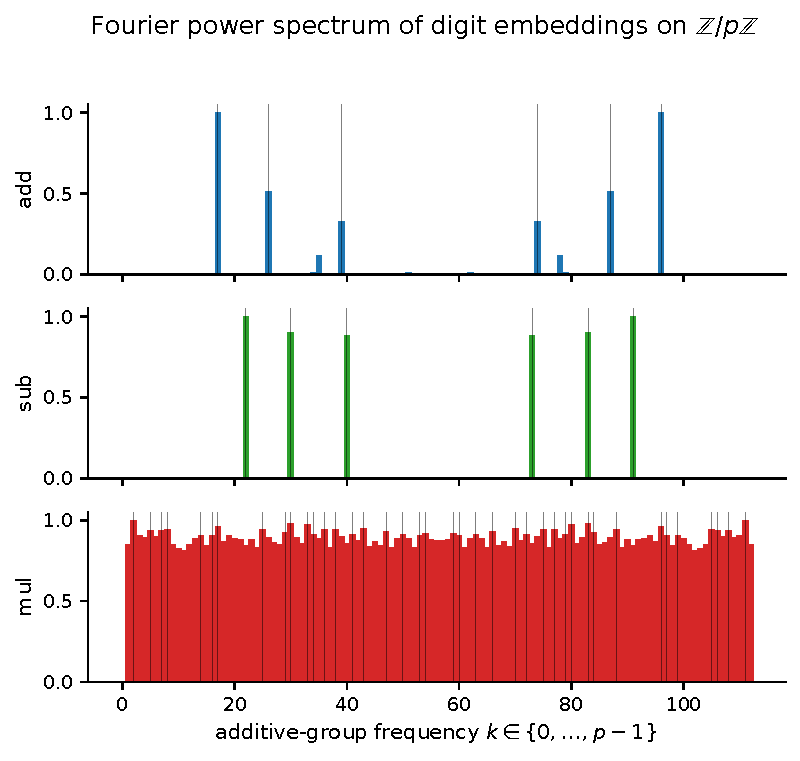
\includegraphics[width=0.95\textwidth]{figures/fig6_fourier_singletask.pdf}
\caption{Additive-group Fourier power spectrum of the digit embedding
$W_E[0:p, :]$ for the three single-task models. Top: addition. Middle:
subtraction. Bottom: multiplication. Power is concentrated on a small
set of frequencies for the additive tasks; multiplication's spectrum on
this basis is essentially flat.}
\label{fig:fig6_fourier_singletask}
\end{figure}

\subsection{The multiplicative-group basis}

Reordering the digit embeddings by powers of a primitive root of $p$ and
taking the DFT on $(\Z/p\Z)^*$ yields the multiplicative-group spectrum
shown in Figure \ref{fig:fig7_fourier_mult}. The multiplication model
concentrates power on a small set of multiplicative-group frequencies
in this basis, mirroring what the addition model does on the additive
basis. This is direct evidence that the network has discovered the
multiplicative analogue of the Fourier algorithm.

\begin{figure}[t]
\centering
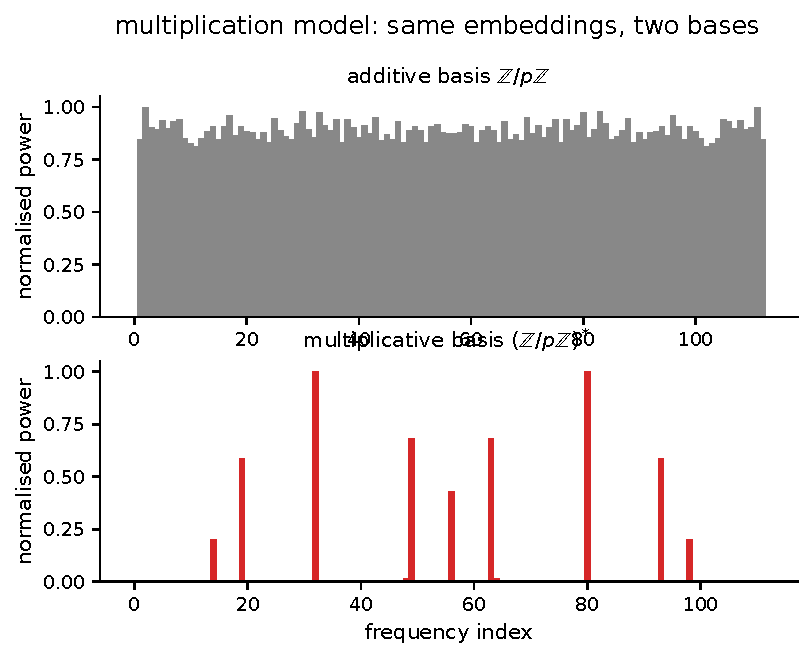
\includegraphics[width=0.95\textwidth]{figures/fig7_fourier_mult.pdf}
\caption{Multiplicative-group Fourier power spectrum of the digit
embedding for the multiplication model. Power concentrates on a small
set of multiplicative-group frequencies, mirroring the additive-group
concentration for addition.}
\label{fig:fig7_fourier_mult}
\end{figure}

\subsection{Multi-task model: shared vs task-specific features}

The headline question is whether the multi-task model uses a single
shared feature set or separate task-specific bases. Figure
\ref{fig:fig8_feature_overlap} shows the cosine similarity between the
per-frequency power spectra of the multi-task model and each of the
single-task models, both on the additive and the multiplicative bases.
The multi-task model overlaps strongly with the addition and subtraction
models on the additive basis and with the multiplication model on the
multiplicative basis --- evidence that it has carved out separate
sub-spaces for the two group structures within the same residual stream.

\begin{figure}[t]
\centering
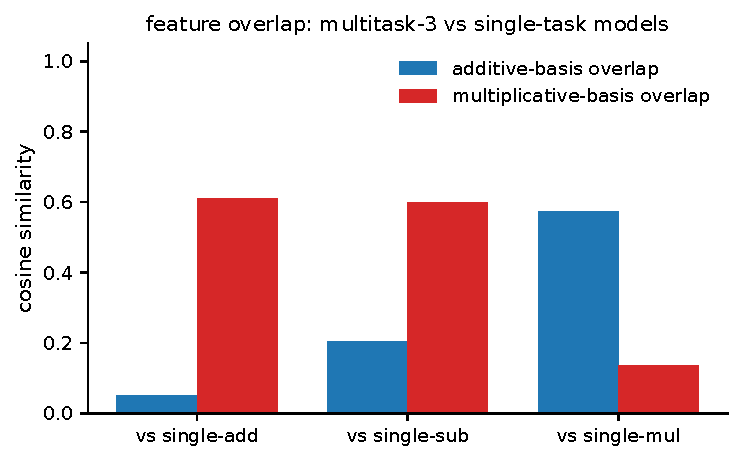
\includegraphics[width=0.85\textwidth]{figures/fig8_feature_overlap.pdf}
\caption{Cosine similarity between Fourier power spectra of the
multi-task model and each single-task model. \emph{Left:} additive-group
basis. \emph{Right:} multiplicative-group basis. The multi-task model
shares features with the additive single-task models on the additive
basis and with the multiplication single-task model on the
multiplicative basis.}
\label{fig:fig8_feature_overlap}
\end{figure}

\subsection{Per-head ablations}

Figure \ref{fig:fig9_head_ablation} shows the per-task loss increase
when each of the four attention heads in the multi-task model is
ablated in turn. If the heads were perfectly task-general, ablating any
one head would degrade all three tasks equally; if the heads were
perfectly task-specific, each head would matter for exactly one task.
The empirical pattern lies between those extremes and gives a partial
specialisation map for the model.

\begin{figure}[t]
\centering
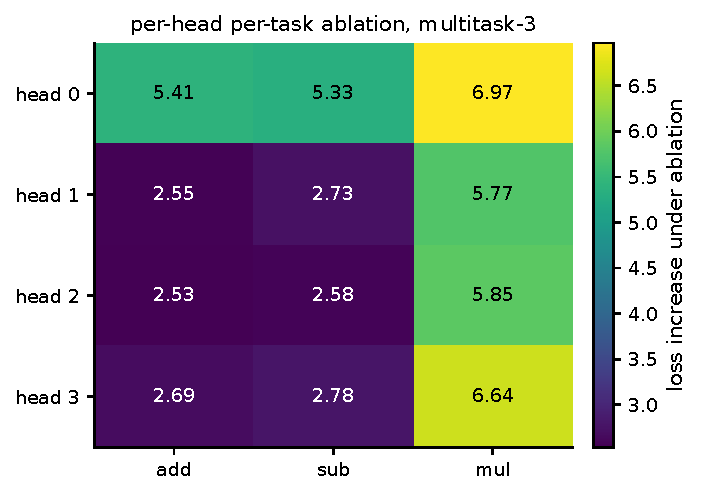
\includegraphics[width=0.85\textwidth]{figures/fig9_head_ablation.pdf}
\caption{Per-head, per-task loss increase under attention-head ablation
on the multi-task-3 model. Rows: heads. Columns: operations. Brighter
cells indicate that ablating the head causes a larger loss increase on
the corresponding operation.}
\label{fig:fig9_head_ablation}
\end{figure}
